\documentclass[twoside,11pt]{article}

% Any additional packages needed should be included after jmlr2e.
% Note that jmlr2e.sty includes epsfig, amssymb, natbib and graphicx,
% and defines many common macros, such as 'proof' and 'example'.
%
% It also sets the bibliographystyle to plainnat; for more information on
% natbib citation styles, see the natbib documentation, a copy of which
% is archived at http://www.jmlr.org/format/natbib.pdf

\usepackage{jmlr2e}

% Definitions of handy macros can go here

\newcommand{\dataset}{{\cal D}}
\newcommand{\fracpartial}[2]{\frac{\partial #1}{\partial  #2}}

% Heading arguments are {volume}{year}{pages}{submitted}{published}{author-full-names}

\jmlrheading{20}{2019}{1-10}{9/19}{10/19}{Sladek, Thompson, Hagerman, and Hansen}

% Short headings should be running head and authors last names

\ShortHeadings{CSCI 447 Project 1}{Sladek, Thompson, Hagerman, and Hansen}
\firstpageno{1}

\begin{document}

\title{Machine Learning Project 2: Design Document}

\author{\name Brandon Sladek \email 
      brandonsladek@gmail.com \\ \addr School of Computing\\ Montana State University\\
       Bozeman, MT 59718, USA
        \AND
        \name Jared Thompson \email j.a.thompson22@gmail.com \\ \addr School of Computing\\ Montana State University\\
       Bozeman, MT 59718, USA
        \AND
        \name Kyle Hagerman \email hagermankyle96@gmail.com \\ \addr School of Computing\\ Montana State University\\
       Bozeman, MT 59718, USA
        \AND
        \name Ryan Hansen \email ryanhansen2222@gmail.com \\ \addr School of Computing\\ Montana State University\\
       Bozeman, MT 59718, USA}
       
\editor{Editor: N/A}

\maketitle

\section{Design Overview}

In this section we present an overview of our proposed architecture for a Python application that does classification using five variants of the k-Nearest-Neighbor algorithm.

    \subsection{Outline}
    The core of our design is based upon a main driver class, ExperimentRunner. This class will instantiate a class for each algorithm implementation that extends a parent class, Algorithms. We chose to create the Algorithms class to provide common tools to each algorithm. This gives our code good reusability. Should we have to add another version of k-Nearest-Neighbor then we will only have to create a new class and add the algorithm specific methods required for its implementation.
    
    The ExperimentRunner will also use the Pandas DataFrame, dataset Preprocessor, and CrossValidator by calling their respective classes. Specifically, the DataAPI class handles creating the Pandas DataFrames and will store each frame. The Preprocessor class will call a general method that analyzes each DataFrame and handles exceptions accordingly. The CrossValidator class will implement a 10-fold cross validation and reserve one tenth of the dataset as a test set for each iteration. The Results class will run analysis on each model's results using two loss functions, 0/1 Loss and Mean Squared Error. 
    
    \subsection{Parameter Tuning}
    The first parameter to be tuned is the value for k from the k-Nearest-Neighbor algorithm, which will be tuned against a performance measure to determine the optimal value needed for classification. The second two parameters to tune are the number of medoids and centroids to be used in PAM and k-means, respectively. Both of which will be iteratively tuned until we find the optimal number that no longer increases our performance. In this respect, one initial assumption that can be made about the number (for K-means and PAM) is that it needs to be at least equal to, or greater than, the number of classes in our data set.
    
    \subsection{Decisions}
    We implemented an Algorithms parent class across all five algorithm classes in order to abstract out methods that can be used across multiple algorithm classes. These three methods are k\_nn(), get\_distance(), and get\_mean(). Here, the difference between the KNN class and the k\_nn() method is that the child class object handles any of the additional data preprocessing and data pulling that needs to be done prior to running k\_nn(). 
    
    In preprocessing, we choose to supplement missing values with randomly generated values in the domain of possible values for that attribute. We chose to include k\_nn() in the parent Algorithm class because some version of nearest neighbor classification is used in all five algorithms. The primary difference is not in the logic, but in the data passed in, and the number chosen for k. Furthermore, all five algorithms use get\_distance() and a get\_means() function, so in order to simplify the overall architecture we included them in the parent class. Finally, as k-means/k-medoids do not necessarily terminate, we choose to implement a hard cap of 100 iterations to guarantee the algorithms end.
    
\section{Experiment}
This section discusses the experimental motivation and general approach for accepting or rejecting our hypothesis for the various data sets and potential k-values.
    
    \subsection{Hypothesis}
    We have a number of different algorithms we want to compare for different scenarios over the course of this experiment. We want to compare performance of our classification scenarios through loss functions. The following table depicts our hypothesis - 
    \begin{table}[h]
\begin{tabular}{ll}
               & \textbf{Performance Rank (1 best, 5 worst)}                                                                                   \\
\textit{k-NN}           & \textbf{2} - aggregate of the whole data set (best with mid range k)                              \\
\textit{Edited k-NN}    & \textbf{1} - constructed for accuracy for the most points (best with higher k)                    \\
\textit{Condensed k-NN} & \textbf{5} - constructed for identifying bad data (best with higher k)                    \\
\textit{k-means}        & \textbf{4} - prone to outliers, and no guarantee clusters form classes (best with low k) \\
\textit{k-medoids}      & \textbf{3} - step above k-means, outlier resistant. (best with low k)                           
\end{tabular}
\end{table}

    \subsection{Approach}
    First, we plan to use Python with the Pandas library to code the algorithms we wish to test \cite{McKinney:2010}. Second, for the sake of consistency, we plan to use 10-fold cross validation to verify our results. In probabilistic experiments, it is possible to get good or bad results due to random chance. Cross validation helps mitigate this problem. In particular, 10-fold cross validation is one of the most common forms of cross validation used in modern machine learning research.

\section{Proposed Analysis}
    Our analysis will compare the performance of each algorithm using two loss functions. We have chosen to use 0/1 Loss and Mean Squared Error.
    
    In our implementation, 0/1 Loss will sum the number of incorrect classifications for each algorithm and average over each of the 10 folds in cross validation. This measurement will be a direct measure of the accuracy of each model, and will be used to rank each accordingly.
    
    We will also implement Mean Squared Error for another look at the accuracy of our models. Because the classification result is a binary measure we will define the loss function to calculate results accordingly. When summing the difference between the expected value and the actual classification, we will add a 0 if the classification was correct and a -1 otherwise. This measure of accuracy averages over the number of points we classified from the test set and averages again over each of the 10 folds. Between both measures of accuracy we will have a clear picture of which model classified data points better for different k-values.

\newpage

\bibliographystyle{ieeetr}
\bibliography{project2_dd_references}
\begin{figure}
    \centering
    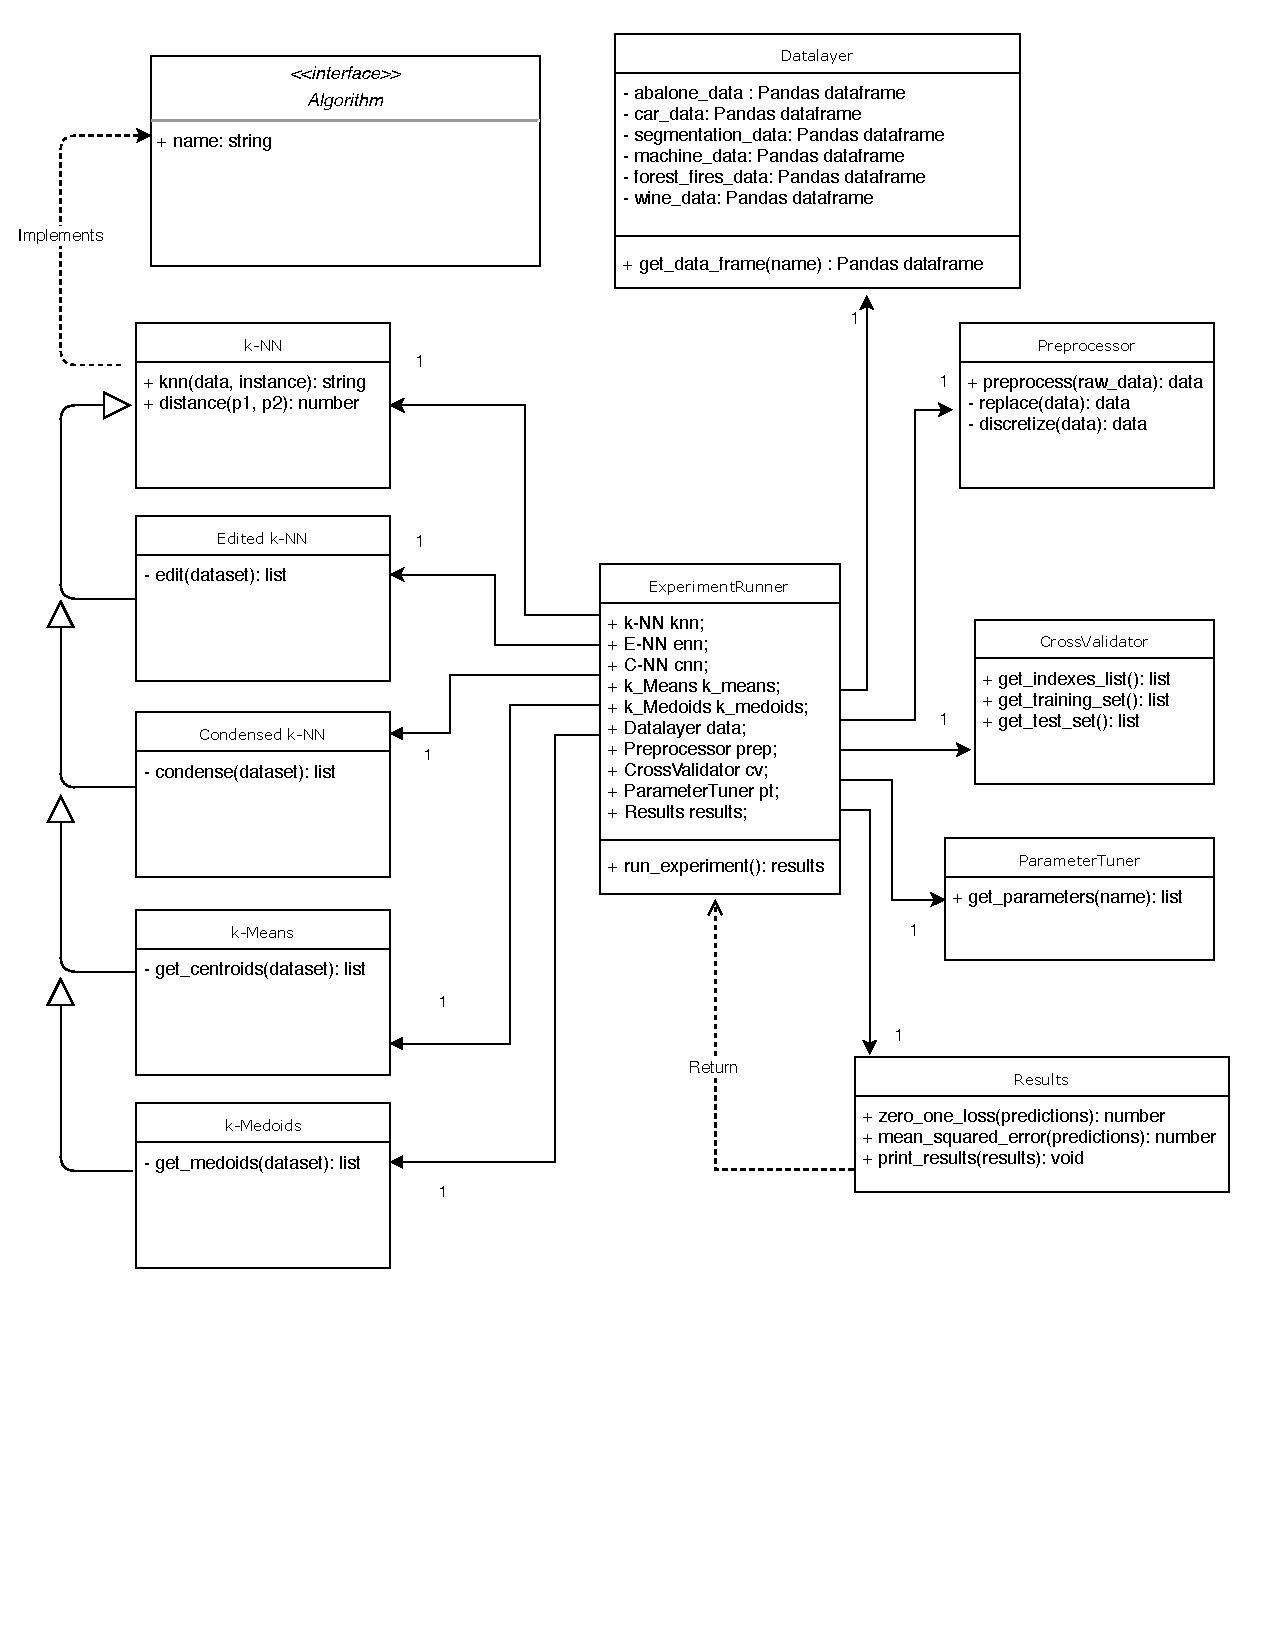
\includegraphics[width=1\textwidth]{ML_Project2_UML.pdf}
    \caption{UML Implementation of k-NN Algorithm Suite}
    \label{fig:my_label}
\end{figure}
\end{document}